% Options for packages loaded elsewhere
\PassOptionsToPackage{unicode}{hyperref}
\PassOptionsToPackage{hyphens}{url}
\PassOptionsToPackage{dvipsnames,svgnames*,x11names*}{xcolor}
%
\documentclass[
  12pt,
]{article}
\usepackage{amsmath,amssymb}
\usepackage{lmodern}
\usepackage{ifxetex,ifluatex}
\ifnum 0\ifxetex 1\fi\ifluatex 1\fi=0 % if pdftex
  \usepackage[T1]{fontenc}
  \usepackage[utf8]{inputenc}
  \usepackage{textcomp} % provide euro and other symbols
\else % if luatex or xetex
  \usepackage{unicode-math}
  \defaultfontfeatures{Scale=MatchLowercase}
  \defaultfontfeatures[\rmfamily]{Ligatures=TeX,Scale=1}
\fi
% Use upquote if available, for straight quotes in verbatim environments
\IfFileExists{upquote.sty}{\usepackage{upquote}}{}
\IfFileExists{microtype.sty}{% use microtype if available
  \usepackage[]{microtype}
  \UseMicrotypeSet[protrusion]{basicmath} % disable protrusion for tt fonts
}{}
\makeatletter
\@ifundefined{KOMAClassName}{% if non-KOMA class
  \IfFileExists{parskip.sty}{%
    \usepackage{parskip}
  }{% else
    \setlength{\parindent}{0pt}
    \setlength{\parskip}{6pt plus 2pt minus 1pt}}
}{% if KOMA class
  \KOMAoptions{parskip=half}}
\makeatother
\usepackage{xcolor}
\IfFileExists{xurl.sty}{\usepackage{xurl}}{} % add URL line breaks if available
\IfFileExists{bookmark.sty}{\usepackage{bookmark}}{\usepackage{hyperref}}
\hypersetup{
  pdftitle={Compositional data analysis for migration studies},
  colorlinks=true,
  linkcolor=Maroon,
  filecolor=Maroon,
  citecolor=Blue,
  urlcolor=blue,
  pdfcreator={LaTeX via pandoc}}
\urlstyle{same} % disable monospaced font for URLs
\usepackage[margin=1in]{geometry}
\usepackage{longtable,booktabs,array}
\usepackage{calc} % for calculating minipage widths
% Correct order of tables after \paragraph or \subparagraph
\usepackage{etoolbox}
\makeatletter
\patchcmd\longtable{\par}{\if@noskipsec\mbox{}\fi\par}{}{}
\makeatother
% Allow footnotes in longtable head/foot
\IfFileExists{footnotehyper.sty}{\usepackage{footnotehyper}}{\usepackage{footnote}}
\makesavenoteenv{longtable}
\usepackage{graphicx}
\makeatletter
\def\maxwidth{\ifdim\Gin@nat@width>\linewidth\linewidth\else\Gin@nat@width\fi}
\def\maxheight{\ifdim\Gin@nat@height>\textheight\textheight\else\Gin@nat@height\fi}
\makeatother
% Scale images if necessary, so that they will not overflow the page
% margins by default, and it is still possible to overwrite the defaults
% using explicit options in \includegraphics[width, height, ...]{}
\setkeys{Gin}{width=\maxwidth,height=\maxheight,keepaspectratio}
% Set default figure placement to htbp
\makeatletter
\def\fps@figure{htbp}
\makeatother
\setlength{\emergencystretch}{3em} % prevent overfull lines
\providecommand{\tightlist}{%
  \setlength{\itemsep}{0pt}\setlength{\parskip}{0pt}}
\setcounter{secnumdepth}{5}
\usepackage{float}
\usepackage{booktabs}
\usepackage{booktabs}
\usepackage{longtable}
\usepackage{array}
\usepackage{multirow}
\usepackage{wrapfig}
\usepackage{float}
\usepackage{colortbl}
\usepackage{pdflscape}
\usepackage{tabu}
\usepackage{threeparttable}
\usepackage{threeparttablex}
\usepackage[normalem]{ulem}
\usepackage{makecell}
\usepackage{xcolor}
\ifluatex
  \usepackage{selnolig}  % disable illegal ligatures
\fi

\title{Compositional data analysis for migration studies}
\author{}
\date{\vspace{-2.5em}}

\begin{document}
\maketitle

\textbf{Authors:} Javier Elío\footnote{Department of Planning, Aalborg University, Copenhagen, Denmark; ORCID: \href{https://orcid.org/0000-0003-0624-2345}{0000-0003-0624-2345}; \href{mailto:javierdem@plan.aau.dk}{\nolinkurl{javierdem@plan.aau.dk}} - \href{mailto:javiereliomedina@gmail.com}{\nolinkurl{javiereliomedina@gmail.com}}},
Marina Georgati\footnote{Department of Planning, Aalborg University, Copenhagen, Denmark; ORCID: \href{https://orcid.org/0000-0001-7794-8308}{0000-0001-7794-8308}; \href{mailto:marinag@plan.aau.dk}{\nolinkurl{marinag@plan.aau.dk}}},
Henning S. Hansen\footnote{Department of Planning, Aalborg University, Copenhagen, Denmark; ORCID: \href{https://orcid.org/0000-0001-7004-0698}{0000-0001-7004-0698}; \href{mailto:hsh@plan.aau.dk}{\nolinkurl{hsh@plan.aau.dk}}},
Carsten Keßler\footnote{Department of Planning, Aalborg University, Copenhagen, Denmark; ORCID: \href{https://orcid.org/0000-0002-9724-820X}{0000-0002-9724-820X}; \href{mailto:kessler@plan.aau.dk}{\nolinkurl{kessler@plan.aau.dk}}}.\\

\textbf{Corresponding author}: Carsten Keßler\\

\hypertarget{prerequisites}{%
\section{Prerequisites}\label{prerequisites}}

The data have been analysed with \textbf{R} (version 4.1.0) and \textbf{Rstudio} (version 1.4.1717). The required packages are automatically checked and installed if needed from CRAN.

Furthermore, we have created our own package for downloading \href{https://kortforsyningen.dk/}{kortforsyningen} data to a local repository directly from R (i.e.~\href{https://github.com/javiereliomedina/dangeo.git}{dangeo}). The package can be downloaded from GitHub:

Although the \emph{kortforsyningen} data are free, we would need to create a \emph{username} and a \emph{password} for getting access to them (you can make it here: \href{https://kortforsyningen.dk/indhold/min-side-0}{``Opret ny bruger''}). By default \textbf{dangeo} looks for credentials on \texttt{.Renviron} as: \texttt{kortforsyningen\_id\ =\ "username"} and \texttt{kortforsyningen\_pwd\ =\ "password"}. You would need to save them with \texttt{usethis::edit\_r\_environ()}:

You would also need to define with \texttt{dangeo\_set\_param()} the local directory where the data are downloaded (\texttt{loc\_dir}). It is defined as \texttt{loc\_dir\ =\ rappdirs::user\_cache\_dir()}, although it can be changed \texttt{loc\_dir\ =\ “./your/local/path”}. The first time a file is downloaded with \texttt{dangeo\_get\_data()}, the process can be time consuming (there are some very big files). However, it will not be downloaded in subsequent calls if the files is already in the local directory (the dataset can be overwritten be setting \texttt{overwrite\ =\ TRUE} on \texttt{dangeo\_get\_data()}). Once we have our \emph{username} and \emph{password}, and we have define the local repository for the data, we can set them on our R-session:

Individual house prices data (from BBR) are not free, and we have save here the summary statistics by parish (i.e.~median value).

Set ggplot theme.

\hypertarget{data}{%
\section{Data}\label{data}}

\hypertarget{spatial-data}{%
\subsection{Spatial data}\label{spatial-data}}

\begin{center}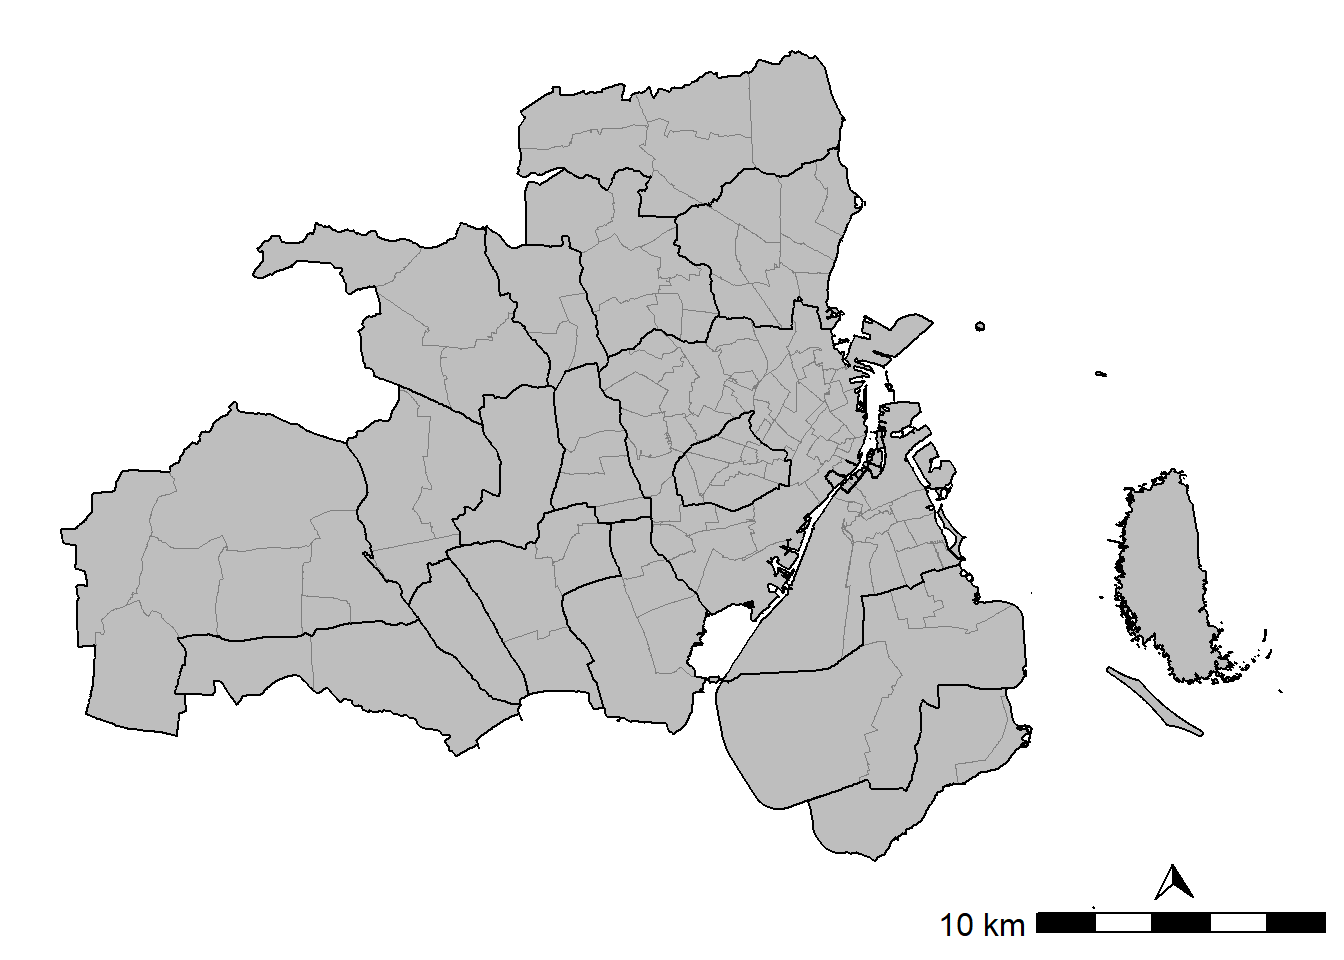
\includegraphics{CoDa_migr_cph_files/figure-latex/fig-cap-reg-prsh-1} \end{center}

\hypertarget{population}{%
\subsection{Population}\label{population}}

Population data in 2020 were uploaded from Denmark Statistics:

\begin{itemize}
\tightlist
\item
  \href{https://www.statbank.dk/statbank5a/SelectVarVal/Define.asp?MainTable=KMSTA001\&PLanguage=1\&PXSId=0\&wsid=cftree}{KMSTA001: Population 1. January by parish, ancestry and National Church}.
\end{itemize}

\hypertarget{house-prices}{%
\subsection{House prices}\label{house-prices}}

House prices in 2020 from BBR.

\hypertarget{analysis}{%
\section{Analysis}\label{analysis}}

\hypertarget{population-1}{%
\subsection{Population}\label{population-1}}

\begin{figure}[H]

{\centering \includegraphics{CoDa_migr_cph_files/figure-latex/fig-pop-parish-dan-1} 

}

\caption{Population distribution}\label{fig:fig-pop-parish-dan}
\end{figure}

\hypertarget{house-prices-1}{%
\subsection{House prices}\label{house-prices-1}}

The total number of residential units used for the analysis is therefore 18764 (Table \ref{tab:tbl-runits-oft-capital}). The summary descriptive statistics of the housing prices are:

House prices by type (removing very low prices; i.e.~\textless1 kDKK/m2, n = 242).

\begin{figure}[H]

{\centering \includegraphics{CoDa_migr_cph_files/figure-latex/fig-runits-oft-type-1} 

}

\caption{Boxplot of residential units in the open free trade by house typr (values have been truncated with house prices >1 kDkk/m2)}\label{fig:fig-runits-oft-type}
\end{figure}

House prices parish (spatial distribution)

\begin{figure}[H]

{\centering 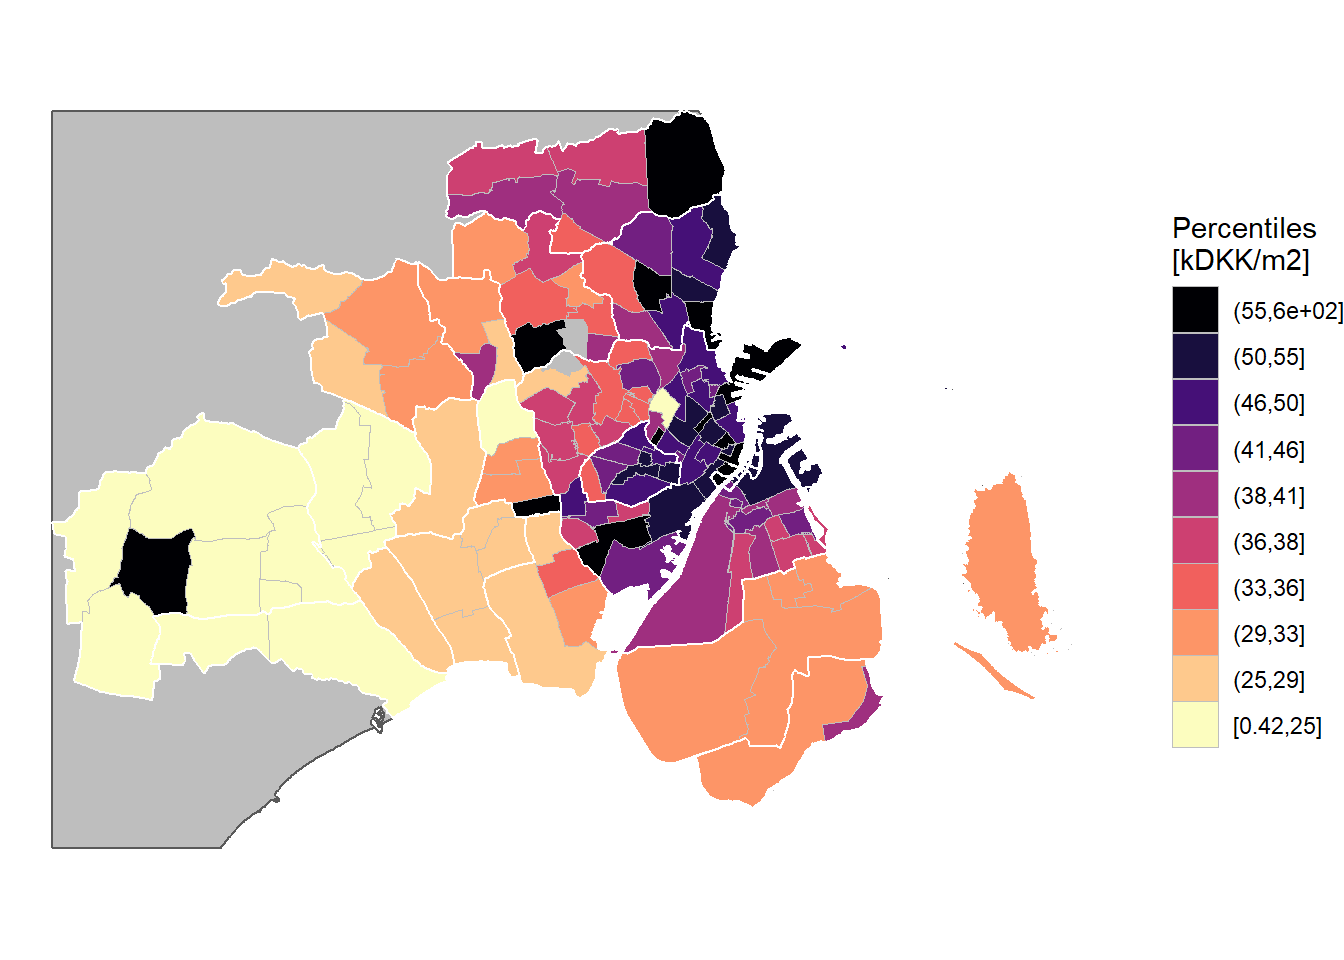
\includegraphics{CoDa_migr_cph_files/figure-latex/fig-prices-runits-parish-b-1} 

}

\caption{Median house prices in the ordinary free trade}\label{fig:fig-prices-runits-parish-b}
\end{figure}

\hypertarget{compositional-data-analysis}{%
\subsection{Compositional data analysis}\label{compositional-data-analysis}}

Ternary plot (there are conflicts between \emph{ggtern} and \emph{ggplot} and we make the ternary plots in a separate project; \url{https://javiereliomedina.github.io/ternary_maps_DK/})

\begin{figure}[H]

{\centering \includegraphics{https://github.com/javiereliomedina/ternary_maps_DK/raw/main/_bookdown_files/ternary_maps_DK_files/figure-html/fig-cap-reg-tern-map-2020-1} 

}

\caption{Population distribution in 2020}\label{fig:fig-tern-pop}
\end{figure}

PCA (with clr transformations). Helps to identify the variables that account the most for the variability of the results and chose the balance. \ldots.

\begin{figure}[H]

{\centering \includegraphics{CoDa_migr_cph_files/figure-latex/prsh-CoDa-PCA-1} 

}

\caption{Biplot of clr transfomation and balance dendrogram}\label{fig:prsh-CoDa-PCA}
\end{figure}

In our cases, with only three variables, our balances are:

\[ b_1 = \sqrt{\frac{2}{3}} * ln(\frac{x_1 x_2}{x_3^2}) \]
\[ b_2 = \sqrt{\frac{1}{2}} * ln(\frac{x_1}{x_2}) \]
Where \(x_1\), \(x_2\), \(x_3\) are the Danes, Western, and Non-wester population in the parish.

We can therefore analyse the spatial autocorrelation of the balances:

\begin{verbatim}
## # A tibble: 2 x 8
##   balance moran_I expectation variance statistic  p.value method     alternative
##   <chr>     <dbl>       <dbl>    <dbl>     <dbl>    <dbl> <chr>      <chr>      
## 1 b1        0.470    -0.00794  0.00312      8.56 5.50e-18 Moran I t~ greater    
## 2 b2        0.542    -0.00794  0.00313      9.84 3.92e-23 Moran I t~ greater
\end{verbatim}

\begin{center}\includegraphics{CoDa_migr_cph_files/figure-latex/prsh-CoDa-moran-local-b1-1} \end{center}

\begin{center}\includegraphics{CoDa_migr_cph_files/figure-latex/prsh-CoDa-moran-local-b2-1} \end{center}

Spatial clusters (k-means cluster) with balances: separate Non-western from Danes and Western citizens.

\begin{center}\includegraphics{CoDa_migr_cph_files/figure-latex/prsh-CoDa-cluster-1} \end{center}

\begin{center}\includegraphics{CoDa_migr_cph_files/figure-latex/prsh-CoDa-cluster-k4-1} \end{center}

\begin{verbatim}
## # A tibble: 4 x 5
##   .cluster pop_dan_pct pop_frgn_wst_pct pop_frgn_nwst_pct pop_total_pct
##   <fct>          <dbl>            <dbl>             <dbl>         <dbl>
## 1 1               80.4            10.2               8.36           100
## 2 2               88.4             4.93              7.11           100
## 3 3               78.8             6.24             14.9            100
## 4 4               63.4             7.15             27.8            100
\end{verbatim}

\begin{figure}[H]

{\centering \includegraphics{CoDa_migr_cph_files/figure-latex/prsh-CoDa-cluster-boxplot-1} 

}

\caption{Cluster characteristics}\label{fig:prsh-CoDa-cluster-boxplot}
\end{figure}

\hypertarget{linear-model}{%
\subsubsection{Linear model}\label{linear-model}}

Links with house prices (zoom the figure to the parishes with median values).

\begin{figure}[H]

{\centering \includegraphics{https://github.com/javiereliomedina/ternary_maps_DK/raw/main/_bookdown_files/ternary_maps_DK_files/figure-html/fig-cap-reg-tern-pop-price-2020-1} 

}

\caption{Median housing prices and popupation distribution by parish}\label{fig:fig-cap-reg-tern-pop-price}
\end{figure}

Linear models with N \textgreater{} 5.

\begin{figure}[H]

{\centering 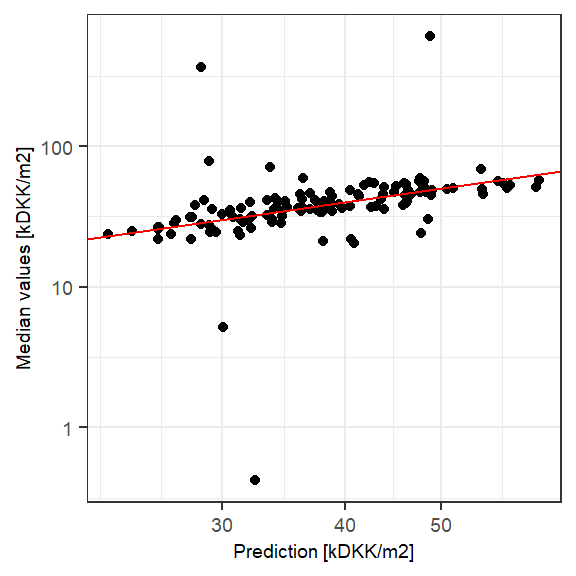
\includegraphics{CoDa_migr_cph_files/figure-latex/fig-prsh-CoDa-house-prices-lm-1} 

}

\caption{Linear model housing prices vs. balances (red line: x = y)}\label{fig:fig-prsh-CoDa-house-prices-lm}
\end{figure}

\hypertarget{acknowledgements}{%
\section*{Acknowledgements}\label{acknowledgements}}
\addcontentsline{toc}{section}{Acknowledgements}

This work has been financed by Aalborg University - AAU (Project: \href{https://www.flow.aau.dk/}{Global flows of migrants and their impact on north European welfare states - FLOW}). The sole responsibility of this publication lies with the authors. AAU is not responsible for any use that may be made of the information contained therein.

\hypertarget{r-session}{%
\section*{R session}\label{r-session}}
\addcontentsline{toc}{section}{R session}

\begin{verbatim}
## R version 4.1.0 (2021-05-18)
## Platform: x86_64-w64-mingw32/x64 (64-bit)
## Running under: Windows 10 x64 (build 19042)
## 
## Matrix products: default
## 
## locale:
## [1] LC_COLLATE=English_United Kingdom.1252 
## [2] LC_CTYPE=English_United Kingdom.1252   
## [3] LC_MONETARY=English_United Kingdom.1252
## [4] LC_NUMERIC=C                           
## [5] LC_TIME=English_United Kingdom.1252    
## 
## attached base packages:
## [1] tools     stats     graphics  grDevices utils     datasets  methods  
## [8] base     
## 
## other attached packages:
##  [1] dangeo_0.0.0.9000     devtools_2.4.2        usethis_2.0.1        
##  [4] tm_0.7-8              NLP_0.2-1             tidytable_0.6.3      
##  [7] tidytext_0.3.1        dplyr_1.0.7           purrr_0.3.4          
## [10] readr_1.4.0           tidyr_1.1.3           tibble_3.1.2         
## [13] tidyverse_1.3.0       table1_1.4.2          viridis_0.6.1        
## [16] viridisLite_0.4.0     units_0.7-2           spdep_1.1-8          
## [19] spData_0.3.10         sp_1.4-5              stars_0.5-3          
## [22] abind_1.4-5           SnowballC_0.7.0       stringr_1.4.0        
## [25] sf_1.0-1              rappdirs_0.3.3        RColorBrewer_1.1-2   
## [28] remotes_2.4.0         rmarkdown_2.9         potential_0.1.0      
## [31] patchwork_1.1.1       opentripplanner_0.3.1 osrm_3.4.1           
## [34] osmextract_0.3.0      mapview_2.10.0        latex2exp_0.5.0      
## [37] knitr_1.33            kableExtra_1.3.4      janitor_2.1.0        
## [40] ggforce_0.3.3         gifski_1.4.3-1        gganimate_1.0.7      
## [43] ggplot2_3.3.5         gtsummary_1.4.2       giscoR_0.2.4         
## [46] ggspatial_1.1.5       furrr_0.2.3           future_1.21.0        
## [49] forcats_0.5.1         dint_2.1.3            danstat_0.1.0        
## [52] data.table_1.14.0     compositions_2.0-2    bookdown_0.22        
## [55] bit64_4.0.5           bit_4.0.4             biscale_0.2.0        
## [58] animation_2.6        
## 
## loaded via a namespace (and not attached):
##   [1] utf8_1.2.1          tidyselect_1.1.1    htmlwidgets_1.5.3  
##   [4] grid_4.1.0          munsell_0.5.0       codetools_0.2-18   
##   [7] withr_2.4.2         colorspace_2.0-2    rstudioapi_0.13    
##  [10] stats4_4.1.0        robustbase_0.93-8   bayesm_3.1-4       
##  [13] listenv_0.8.0       labeling_0.4.2      slam_0.1-48        
##  [16] polyclip_1.10-0     farver_2.1.0        rprojroot_2.0.2    
##  [19] coda_0.19-4         parallelly_1.27.0   LearnBayes_2.15.1  
##  [22] vctrs_0.3.8         generics_0.1.0      xfun_0.24          
##  [25] R6_2.5.0            isoband_0.2.5       cachem_1.0.5       
##  [28] assertthat_0.2.1    scales_1.1.1        gtable_0.3.0       
##  [31] globals_0.14.0      lwgeom_0.2-6        processx_3.5.2     
##  [34] rlang_0.4.11        systemfonts_1.0.2   splines_4.1.0      
##  [37] broom_0.7.8         yaml_2.2.1          modelr_0.1.8       
##  [40] crosstalk_1.1.1     backports_1.2.1     tokenizers_0.2.1   
##  [43] tensorA_0.36.2      ellipsis_0.3.2      raster_3.4-13      
##  [46] proxy_0.4-26        sessioninfo_1.1.1   Rcpp_1.0.7         
##  [49] base64enc_0.1-3     progress_1.2.2      classInt_0.4-3     
##  [52] ps_1.6.0            prettyunits_1.1.1   deldir_0.2-10      
##  [55] haven_2.4.1         fs_1.5.0            leafem_0.1.6       
##  [58] magrittr_2.0.1      gmodels_2.18.1      reprex_2.0.0       
##  [61] pkgload_1.2.1       hms_1.1.0           evaluate_0.14      
##  [64] leaflet_2.0.4.1     readxl_1.3.1        gridExtra_2.3      
##  [67] testthat_3.0.4      compiler_4.1.0      KernSmooth_2.23-20 
##  [70] gt_0.3.0            crayon_1.4.1        htmltools_0.5.1.1  
##  [73] Formula_1.2-4       expm_0.999-6        lubridate_1.7.10   
##  [76] DBI_1.1.1           tweenr_1.0.2        dbplyr_2.1.1       
##  [79] MASS_7.3-54         broom.helpers_1.3.0 boot_1.3-28        
##  [82] Matrix_1.3-4        cli_3.0.1           gdata_2.18.0       
##  [85] parallel_4.1.0      pkgconfig_2.0.3     xml2_1.3.2         
##  [88] svglite_2.0.0       webshot_0.5.2       rvest_1.0.0        
##  [91] snakecase_0.11.0    janeaustenr_0.1.5   callr_3.7.0        
##  [94] digest_0.6.27       cellranger_1.1.0    curl_4.3.2         
##  [97] gtools_3.9.2        satellite_1.0.2     lifecycle_1.0.0    
## [100] nlme_3.1-152        jsonlite_1.7.2      desc_1.3.0         
## [103] fansi_0.5.0         pillar_1.6.1        lattice_0.20-44    
## [106] fastmap_1.1.0       httr_1.4.2          DEoptimR_1.0-9     
## [109] pkgbuild_1.2.0      survival_3.2-11     glue_1.4.2         
## [112] png_0.1-7           class_7.3-19        stringi_1.6.2      
## [115] memoise_2.0.0       e1071_1.7-7
\end{verbatim}

\end{document}
